\section{Results and Discussion}
\label{sec:results}
    This section presents an evaluation of our crash reproduction approach, focusing on its performance across various 
    genetic operators. We conducted experiments using three mutation operators—inversion, random, and swap—and two 
    crossover operators, namely single-point and uniform. To illustrate the fitness evolution achieved by each 
    combination of these genetic operators, we refer to Figures \ref{fig:beacon:1} through \ref{fig:beacon:4}. Our 
    analysis covers two test cases: \texttt{TC1} and \texttt{TC2}. The performance results for \texttt{TC1} are detailed 
    in Figures \ref{fig:beacon:1} and \ref{fig:beacon:3}, while those for \texttt{TC2} are depicted in Figures 
    \ref{fig:beacon:2} and \ref{fig:beacon:4}. These results provide insights into the efficacy of different genetic 
    operator combinations in the context of crash reproduction.

    \begin{figure}[ht!]
        \centering
        \begin{subfigure}{0.45\textwidth}
            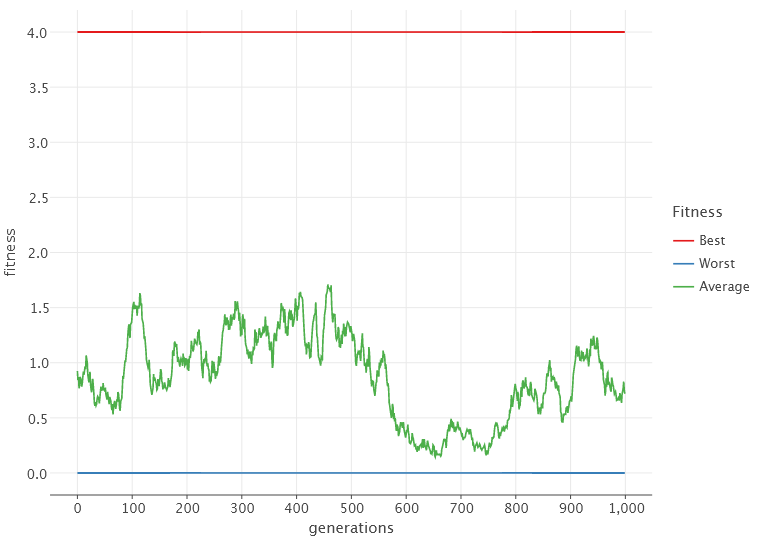
\includegraphics[width=\textwidth]{img/beacon_sp_inv_1.png}
            \caption{Inversion Mutation with a Single Point Crossover}
            \label{fig:beacon:1:inversion}
        \end{subfigure}
        \begin{subfigure}{0.45\textwidth}
            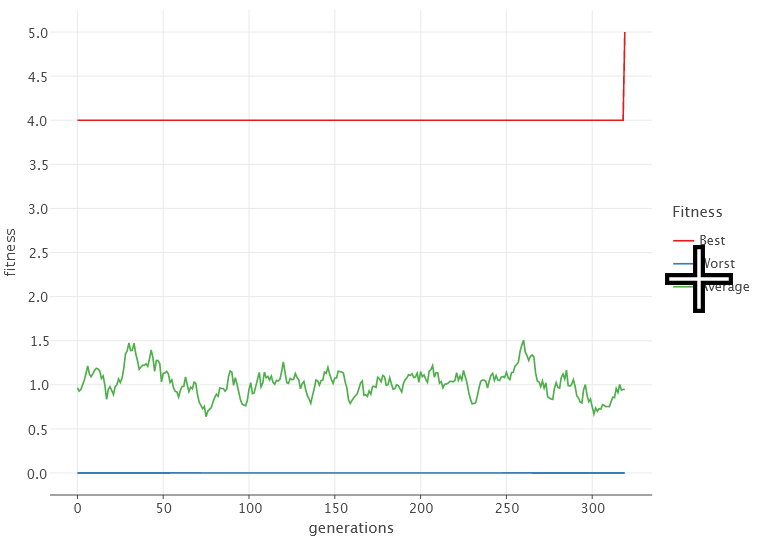
\includegraphics[width=\textwidth]{img/beacon_sp_random_1.png}
            \caption{Random Mutation with a Single Point Crossover}
            \label{fig:beacon:1:random}
        \end{subfigure}
        \begin{subfigure}{0.45\textwidth}
            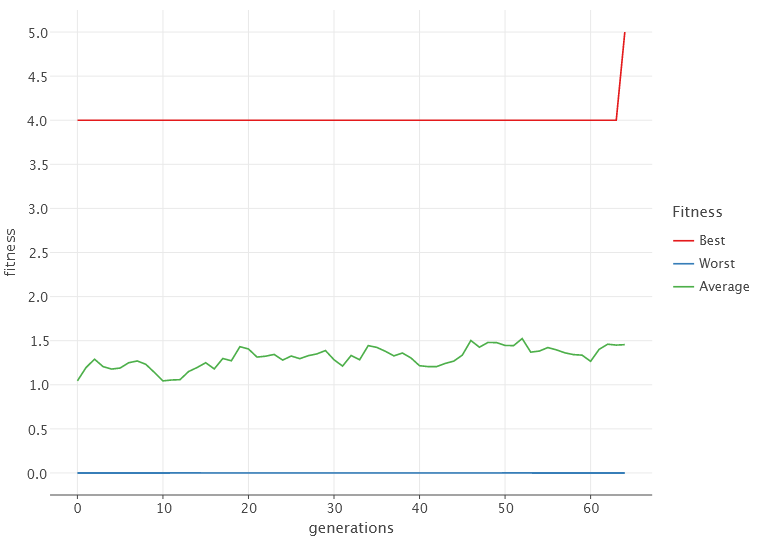
\includegraphics[width=\textwidth]{img/beacon_sp_swap_1.png}
            \caption{Swap Mutation with a Single Point Crossover}
            \label{fig:beacon:1:swap}
        \end{subfigure}
        \caption{Comparison of the three genetic operators on the \texttt{TC1} test case.}
        \label{fig:beacon:1}
    \end{figure}
    
    \begin{figure}[ht!]
        \centering
        \begin{subfigure}{0.45\textwidth}
            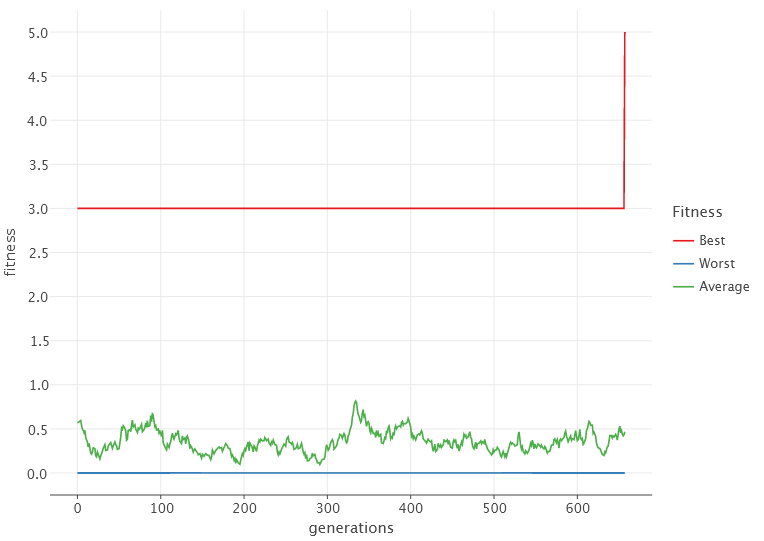
\includegraphics[width=\textwidth]{img/beacon_sp_inv_2.png}
            \caption{Inversion Mutation with a Single Point Crossover}
            \label{fig:beacon:2:inversion}
        \end{subfigure}
        \begin{subfigure}{0.45\textwidth}
            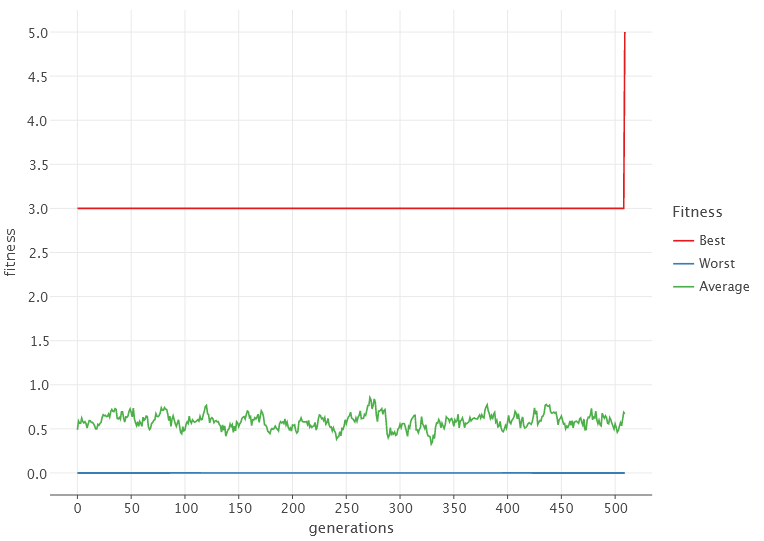
\includegraphics[width=\textwidth]{img/beacon_sp_random_2.png}
            \caption{Random Mutation with a Single Point Crossover}
            \label{fig:beacon:2:random}
        \end{subfigure}
        \begin{subfigure}{0.45\textwidth}
            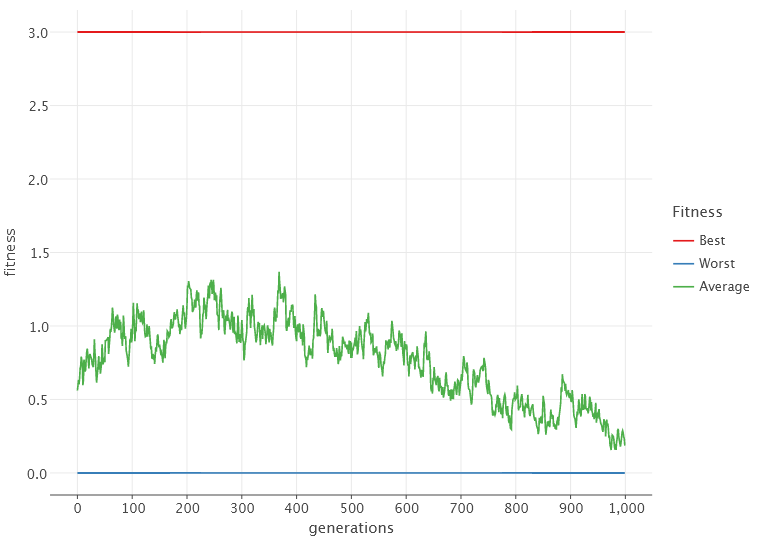
\includegraphics[width=\textwidth]{img/beacon_sp_swap_2.png}
            \caption{Swap Mutation with a Single Point Crossover}
            \label{fig:beacon:2:swap}
        \end{subfigure}
        \caption{Comparison of the three genetic operators on the \texttt{TC2} test case.}
        \label{fig:beacon:2}
    \end{figure}

    \begin{figure}[ht!]
        \centering
        \begin{subfigure}{0.45\textwidth}
            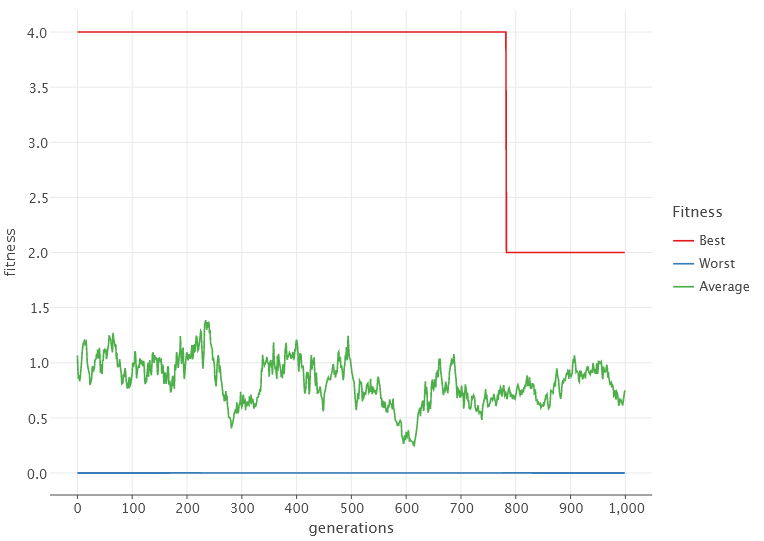
\includegraphics[width=\textwidth]{img/beacon_uniform_inv_1.png}
            \caption{Inversion Mutation with a Uniform Crossover}
            \label{fig:beacon:3:inversion}
        \end{subfigure}
        \begin{subfigure}{0.45\textwidth}
            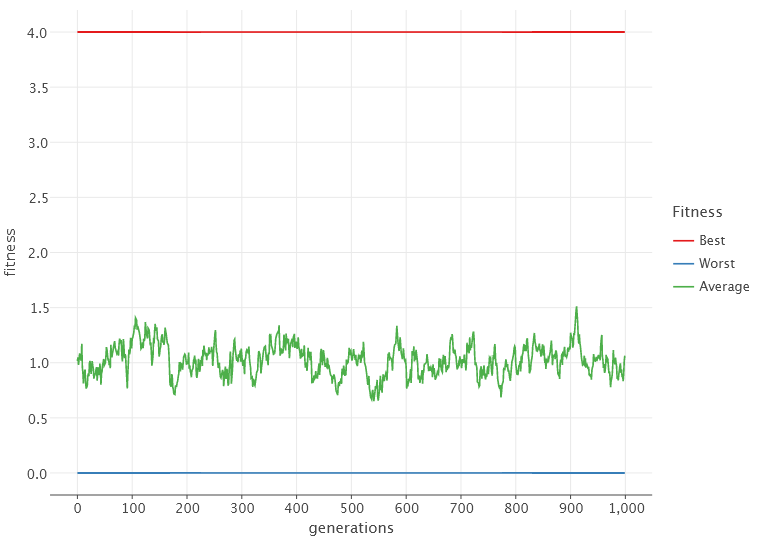
\includegraphics[width=\textwidth]{img/beacon_uniform_random_1.png}
            \caption{Random Mutation with a Uniform Crossover}
            \label{fig:beacon:3:random}
        \end{subfigure}
        \begin{subfigure}{0.45\textwidth}
            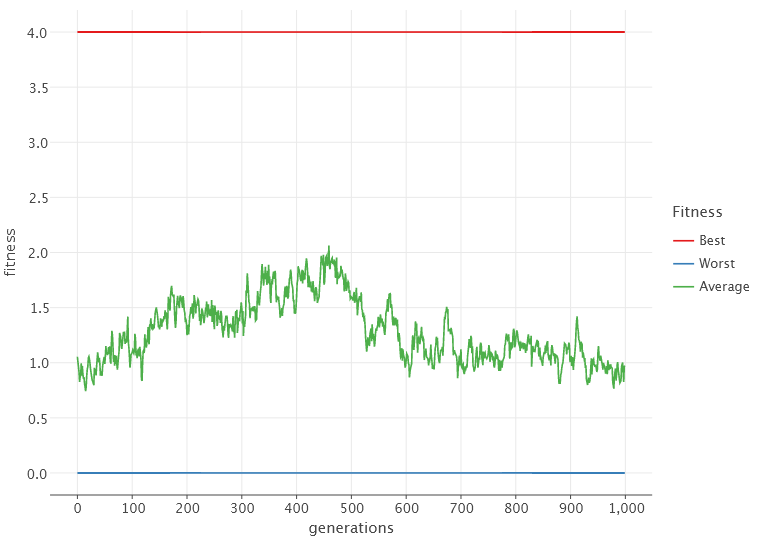
\includegraphics[width=\textwidth]{img/beacon_uniform_swap_1.png}
            \caption{Swap Mutation with a Uniform Crossover}
            \label{fig:beacon:3:swap}
        \end{subfigure}
        \caption{Comparison of the three genetic operators on the \texttt{TC1} test case.}
        \label{fig:beacon:3}
    \end{figure}

    \begin{figure}[ht!]
        \centering
        \begin{subfigure}{0.45\textwidth}
            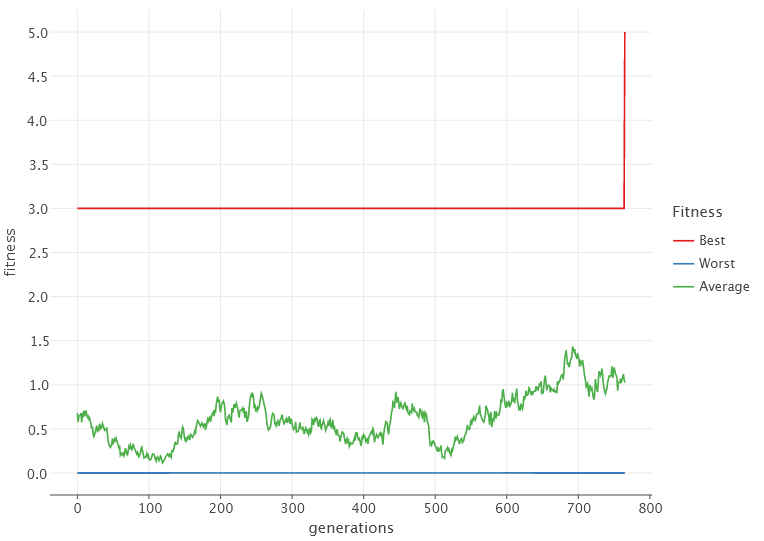
\includegraphics[width=\textwidth]{img/beacon_uniform_inv_2.png}
            \caption{Inversion Mutation with a Uniform Crossover}
            \label{fig:beacon:4:inversion}
        \end{subfigure}
        \begin{subfigure}{0.45\textwidth}
            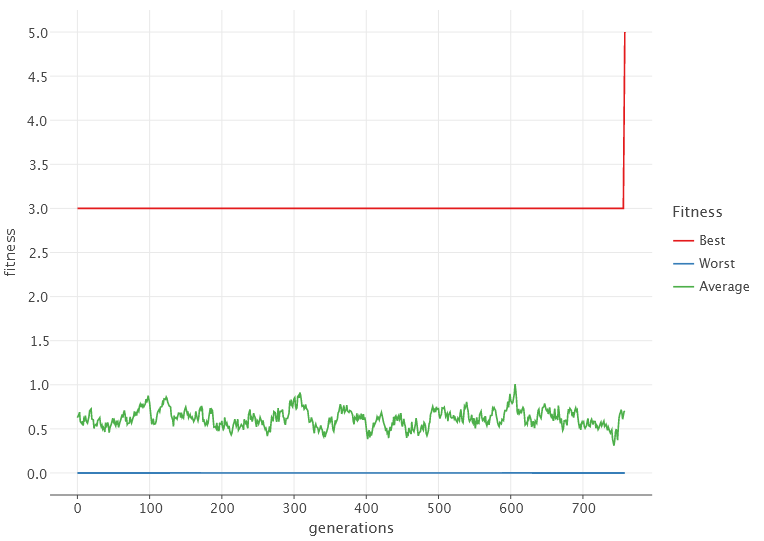
\includegraphics[width=\textwidth]{img/beacon_uniform_random_2.png}
            \caption{Random Mutation with a Uniform Crossover}
            \label{fig:beacon:4:random}
        \end{subfigure}
        \begin{subfigure}{0.45\textwidth}
            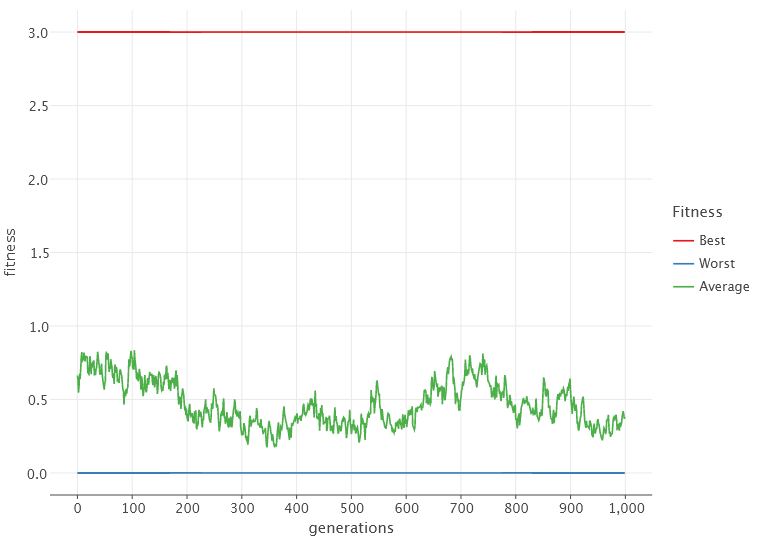
\includegraphics[width=\textwidth]{img/beacon_uniform_swap_2.png}
            \caption{Swap Mutation with a Uniform Crossover}
            \label{fig:beacon:4:swap}
        \end{subfigure}
        \caption{Comparison of the three genetic operators on the \texttt{TC2} test case.}
        \label{fig:beacon:4}
    \end{figure}

    The experimental results demonstrate varied performances among different genetic operators in the context of crash 
    reproduction. Specifically, for test case \texttt{TC1}, the inversion and swap mutation operators paired with 
    single-point crossover achieved the target fitness value of 5.0, whereas the random mutation operator did not. In 
    contrast, when utilizing uniform crossover, none of the operator combinations attained the fitness goal of 5.0. For 
    \texttt{TC2}, both inversion and random mutation operators with single-point crossover reached the target fitness, 
    while the swap mutation operator fell short. However, using uniform crossover, the inversion and swap mutation 
    operators were successful in achieving the fitness target, unlike the random mutation operator.

    These findings imply that the effectiveness of genetic operators significantly depends on the specific test case. In 
    \texttt{TC1}, inversion and swap mutation operators outperform the random mutation operator, while in \texttt{TC2}, 
    inversion and random mutation operators show superior performance compared to the swap mutation operator. 
    Additionally, the uniform crossover operator generally underperforms relative to the single-point crossover in crash 
    reproduction tasks.

    There was no noticeable trend in average fitness improvement over time, suggesting that the fitness function might 
    not be optimally aligned with the crash reproduction problem. This lack of convergence on a solution could be due to 
    the fitness function's inability to effectively differentiate solutions nearing the target fitness value.

    The outcomes might also indicate limitations in the simplified LGP (Linear Genetic Programming) implementation used 
    for this project. A more advanced LGP implementation or a Multi-Objective Genetic Programming (MOGP) approach might 
    yield better results. MOGP could optimize both the target fitness value and the solution's instruction count, 
    potentially leading to solutions that are both close to the desired fitness value and have fewer instructions, thus 
    more likely representing practical crash reproduction solutions.

    Given these insights, we conclude that a statistical analysis of the results is not necessary, as the current 
    findings do not provide a conclusive basis for such an analysis.
